\begin{figure*}[t]
\centering
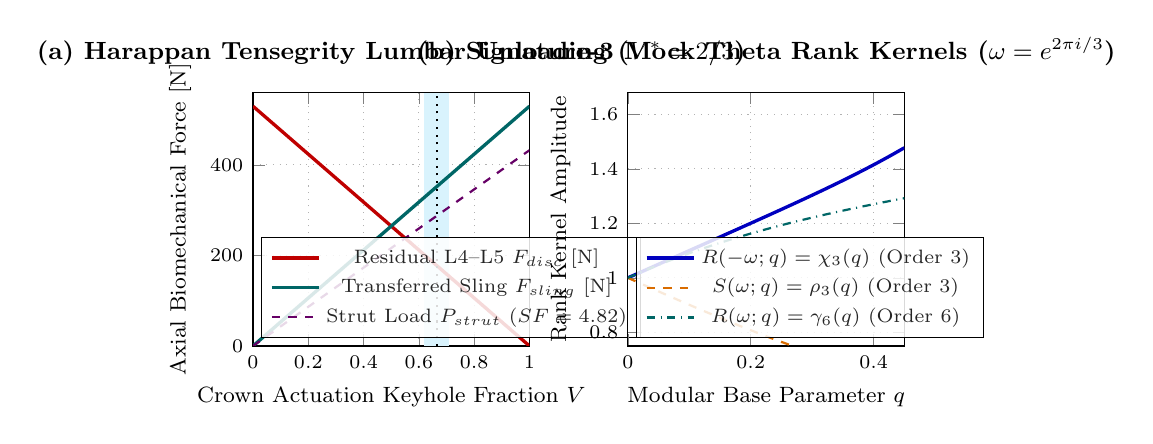
\begin{tikzpicture}
  % --- PANEL (a): Harappan Tensegrity Lumbar Unloading (V* = 34/51 = 2/3) ---
  \begin{axis}[
    name=plotA,
    width=0.42\textwidth,
    height=4.8cm,
    title={\textbf{(a) Harappan Tensegrity Lumbar Unloading (\ensuremath{V^*=2/3})}},
    xlabel={Crown Actuation Keyhole Fraction \ensuremath{V}},
    ylabel={Axial Biomechanical Force [N]},
    xmin=0.0, xmax=1.0,
    ymin=0, ymax=560,
    grid=both,
    grid style={dotted, gray!60},
    legend pos=south west,
    legend style={font=\scriptsize, fill=white, fill opacity=0.85},
    title style={font=\small},
    label style={font=\footnotesize},
    tick label style={font=\scriptsize}
  ]
    \fill[cyan!15] (axis cs:0.62,0) rectangle (axis cs:0.71,560);
    \addplot[domain=0:1, samples=100, red!75!black, very thick] {529.74*(1 - x)};
    \addlegendentry{Residual L4--L5 \ensuremath{F_{\text{disc}}} [N]}
    \addplot[domain=0:1, samples=100, teal!80!black, very thick] {529.74*x};
    \addlegendentry{Transferred Sling \ensuremath{F_{\text{sling}}} [N]}
    \addplot[domain=0:1, samples=100, dashed, violet!80!black, thick] {529.74*x * 2 / (3 * 0.81650)};
    \addlegendentry{Strut Load \ensuremath{P_{\text{strut}}} (\ensuremath{\text{SF}=4.82})}
    \draw[dotted, thick, black] (axis cs:0.6667,0) -- (axis cs:0.6667,560);
  \end{axis}

  % --- PANEL (b): Signature-3 Ramanujan Mock Theta Rank Kernels ---
  \begin{axis}[
    at={(plotA.south east)},
    anchor=south west,
    xshift=1.25cm,
    width=0.42\textwidth,
    height=4.8cm,
    title={\textbf{(b) Signature-3 Mock Theta Rank Kernels (\ensuremath{\omega=e^{2\pi i/3}})}},
    xlabel={Modular Base Parameter \ensuremath{q}},
    ylabel={Rank Kernel Amplitude},
    xmin=0.0, xmax=0.45,
    ymin=0.75, ymax=1.68,
    grid=both,
    grid style={dotted, gray!60},
    legend pos=south west,
    legend style={font=\scriptsize, fill=white, fill opacity=0.85},
    title style={font=\small},
    label style={font=\footnotesize},
    tick label style={font=\scriptsize}
  ]
    \addplot[domain=0:0.45, samples=100, blue!75!black, very thick] {1 + x/(1+x^3) + x^4*(1+x)*(1+x^2)/((1+x^3)*(1+x^6))};
    \addlegendentry{\ensuremath{R(-\omega;q) = \chi_3(q)} (Order 3)}
    \addplot[domain=0:0.45, samples=100, dashed, orange!85!black, thick] {(1-x)/(1-x^3) + x^4*(1-x)*(1-x^3)/((1-x^3)*(1-x^9))};
    \addlegendentry{\ensuremath{S(\omega;q) = \rho_3(q)} (Order 3)}
    \addplot[domain=0:0.45, samples=100, dashdotted, teal!80!black, thick] {1 + x*(1-x)/(1-x^3) + x^4*(1-x)*(1-x^2)/((1-x^3)*(1-x^6))};
    \addlegendentry{\ensuremath{R(\omega;q) = \gamma_6(q)} (Order 6)}
  \end{axis}
\end{tikzpicture}
\caption{\textbf{Page-1 Phase-Space Verification (v4.1.1).} \textbf{(a)} Closed-loop Harappan Tensegrity biomechanical force partition across the $V^* = 34/51 = 2/3$ Avogadro Lagrangian keyhole for an $80.0\text{ kg}$ operator ($W_{\text{torso}} = 529.74\text{ N}$), transferring $F_{\text{sling}} = 353.16\text{ N}$ ($66.67\%$) into the 9-tendon braided jute network and reducing residual L4--L5 compression to $F_{\text{disc}} = 176.58\text{ N}$ with Euler buckling safety factor $\text{SF} = 4.82$. \textbf{(b)} Signature-3 specialization of rank kernels $R(z;q)$ and $S(z;q)$ at Eisenstein cube roots of unity $z = \mp\omega$ ($\omega = e^{2\pi i/3}$), recovering $\chi_3(q)$, $\rho_3(q)$, and $\gamma_6(q)$ alongside the $1729 \leftrightarrow 9271$ multiplicative mirror lock $(36+63)^2 = 9801$.}
\label{fig:dandelion_phase_space}
\end{figure*}
